\documentclass[aspectratio=169, 11pt]{beamer}

% --- Packages & Setup ---
\usepackage[utf8]{inputenc}
\usepackage[T1]{fontenc}
\usepackage{helvet}
\renewcommand{\familydefault}{\sfdefault}
\usepackage{xcolor}
\usepackage{booktabs}
\usepackage{array}
\usepackage{graphicx}
\usepackage{amsmath,amssymb}
\usepackage{adjustbox}
\usepackage{tikz}
\usetikzlibrary{calc,arrows.meta,positioning}
\usepackage{pgfplots}
\pgfplotsset{compat=1.18}

\graphicspath{{../}{./}}

\newcolumntype{C}[1]{>{\centering\arraybackslash}p{#1}}

% Image slot for the before/after slide: replace the \fbox with
% \includegraphics[width=\linewidth,height=3.2cm,keepaspectratio]{<file>}
\newcommand{\imgslot}[1]{%
    \begin{minipage}[c]{0.205\textwidth}
        \centering
        {\scriptsize\textbf{#1}}\\[3pt]
        \fbox{\begin{minipage}[c][3.2cm]{0.9\linewidth}
            \centering {\tiny [Insert image:\\#1]}
        \end{minipage}}
    \end{minipage}}

% --- Branding Colors ---
\definecolor{amritaMaroon}{HTML}{A4123F}
\definecolor{maroonDark}{HTML}{6E0B2A}
\definecolor{maroonTint}{HTML}{F6E8EC}
\definecolor{roseMid}{HTML}{D9A3B4}
\definecolor{inkDark}{HTML}{2B2B2B}
\definecolor{slateGrey}{HTML}{6B6B6B}
\definecolor{goldAccent}{HTML}{C98A1E}

% --- Theme Setup ---
\usetheme{Madrid}
\usecolortheme[named=amritaMaroon]{structure}
\setbeamertemplate{navigation symbols}{}
\setbeamertemplate{footline}[frame number]

% --- Diagram styles ---
\tikzset{
  box/.style={rounded corners=3pt, align=center, font=\small, inner sep=4pt, minimum height=1.05cm},
  dark/.style={box, fill=inkDark, text=white},
  maroon/.style={box, fill=amritaMaroon, text=white},
  deep/.style={box, fill=maroonDark, text=white},
  grey/.style={box, fill=slateGrey, text=white},
  term/.style={box, fill=roseMid, text=inkDark},
  flow/.style={-{Stealth[length=2.2mm]}, line width=0.9pt, color=slateGrey},
  panel/.style={rounded corners=6pt, line width=1.4pt},
}

\begin{document}

% =========================================================================
% TITLE SLIDE (Research-Based Project)
% =========================================================================
\begin{frame}
    \begin{tikzpicture}[remember picture,overlay]
        \node[fill=amritaMaroon, text=white, font=\bfseries\footnotesize, anchor=north east, rounded corners=2pt, inner sep=5pt]
        at ($(current page.north east) + (-0.2cm,-0.2cm)$)
        {Type 1: Research Project};
    \end{tikzpicture}

    \centering
    \includegraphics[width=2.8cm]{logo.png}
    \vspace{0.1cm}

    {\large \textbf{\textcolor{amritaMaroon}{DiffShield: Protecting Face Photos from Diffusion-Model Editing}}} \\
    \vspace{0.05cm}
    {\footnotesize \textbf{23CSE498 -- Project Phase II (External Review)} \quad | \quad \textbf{Team Number: 15}} \\
    \vspace{0.15cm}

    \begin{table}
        \centering
        \footnotesize
        \renewcommand{\arraystretch}{1.05}
        \begin{tabular}{|c|c|l|}
            \hline
            \textbf{S.No} & \textbf{Register Number} & \textbf{Student Name} \\
            \hline
            1 & CB.SC.U4CSE23437 & Pranav Kishan T Y \\
            \hline
            2 & CB.SC.U4CSE23519 & Venkatesh K \\
            \hline
            3 & CB.SC.U4CSE23536 & Narain B K \\
            \hline
            4 & CB.SC.U4CSE23539 & Karthikeyan P G \\
            \hline
            5 & CB.SC.U4CSE23556 & Varun Raj V \\
            \hline
        \end{tabular}
    \end{table}
    \vspace{0.1cm}

    {\footnotesize Guide: \textbf{Dr. Shanmuga Priya S}, Assistant Professor, Department of CSE} \\
    \vspace{0.1cm}
    {\scriptsize \today}
\end{frame}

% =========================================================================
% GUIDE APPROVAL EMAIL CONFIRMATION (Mandatory)
% =========================================================================
\begin{frame}{Guide Review \& Submission Approval}
    \framesubtitle{Confirmation of Project Review and Approval from Guide}
    \centering
    % Replace the box below with:  \includegraphics[width=0.94\textwidth,height=5.4cm,keepaspectratio]{guide_approval.png}
    \fbox{\begin{minipage}[c][5.4cm]{0.94\textwidth}
        \centering
        \textbf{[Insert Screenshot of Guide Approval Email Here]} \\[0.3cm]
        {\footnotesize [Mandatory: Attach a clear, readable screenshot of the email received from your project guide approving this presentation and final review submission]}
    \end{minipage}}
\end{frame}

\section{Problem \& Solution Design}

% --- 1. PROBLEM DEFINITION & RESEARCH MOTIVATION ---
\begin{frame}{1. Problem Definition \& Research Motivation}
    \framesubtitle{Problem Statement, Identified Literature Gap \& Objectives}
    \scriptsize
    \begin{block}{Problem Statement}
        \begin{itemize}
            \item \textbf{Core Research Problem:} diffusion editors can turn any posted face photo into a convincing fake of that person. Can an invisible perturbation ($\le 4/255$ per pixel), added before posting, stop edits from preserving the person's identity?
            \item \textbf{Domain Context:} non-consensual deepfakes are cheap to make; a defence must run offline, stay invisible and survive cleanup (JPEG, resizing, diffusion denoising).
        \end{itemize}
    \end{block}

    \begin{block}{Existing Limitations \& Research Gap}
        \begin{itemize}
            \item \textbf{Summary of Existing Approaches:} PhotoGuard and Mist attack the Stable Diffusion encoder / UNet; Glaze and Anti-DreamBooth target style mimicry and fine-tuning; most use 8--16/255 budgets and image-quality metrics.
            \item \textbf{Identified Research Gap:} little evidence that protection removes \emph{identity} (measured by a face recogniser), survives purification such as DiffPure, and stays invisible on \emph{every} photo.
        \end{itemize}
    \end{block}

    \begin{block}{Research Objectives}
        \begin{itemize}
            \item \textbf{Objective 1 -- Invisibility:} PSNR $\ge$ 38 dB and SSIM $\ge$ 0.95 on every one of the 100 test photos, no pixel changed by more than 4/255.
            \item \textbf{Objective 2 -- Protection:} protection success rate (PSR, judged by ArcFace) clearly above unprotected photos and random noise, with paired 95\% CIs excluding zero; compared with PhotoGuard and Mist.
            \item \textbf{Objective 3 -- Robustness:} protection after common cleanups and across several editors, incl.\ some never used while making the protection; reproducible protocol.
        \end{itemize}
    \end{block}
\end{frame}

% --- 2. PROPOSED METHODOLOGY & OVERALL WORKFLOW ---
\begin{frame}{2. Proposed Methodology \& Overall Workflow}
    \framesubtitle{End-to-End Research Methodology / System Workflow Architecture}
    \centering
    \begin{adjustbox}{max width=\linewidth, max height=5.55cm}
    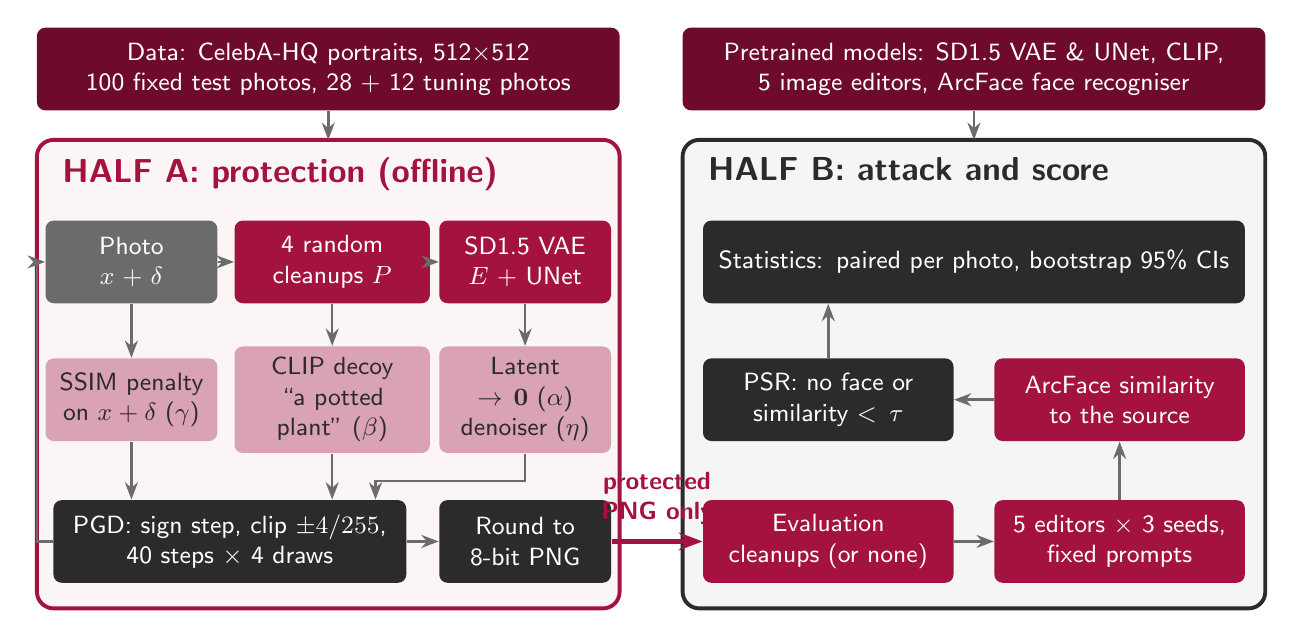
\begin{tikzpicture}
        % top inputs
        \node[deep, minimum width=7.4cm] (data) at (3.9,7.05) {Data: CelebA-HQ portraits, 512$\times$512\\100 fixed test photos, 28 + 12 tuning photos};
        \node[deep, minimum width=7.4cm] (models) at (12.1,7.05) {Pretrained models: SD1.5 VAE \& UNet, CLIP,\\5 image editors, ArcFace face recogniser};

        % panels
        \draw[panel, amritaMaroon, fill=maroonTint!45] (0.2,0.2) rectangle (7.6,6.15);
        \draw[panel, inkDark, fill=black!4] (8.4,0.2) rectangle (15.8,6.15);
        \node[anchor=north west, font=\bfseries\large, text=amritaMaroon] at (0.4,6.05) {HALF A: protection (offline)};
        \node[anchor=north west, font=\bfseries\large, text=inkDark] at (8.6,6.05) {HALF B: attack and score};

        % Half A, row 1
        \node[grey,  minimum width=2.1cm, text width=1.9cm] (x)   at (1.4,4.6) {Photo\\$x+\delta$};
        \node[maroon,minimum width=2.4cm, text width=2.2cm] (cl)  at (3.95,4.6) {4 random cleanups $P$};
        \node[maroon,minimum width=2.1cm, text width=1.9cm] (enc) at (6.4,4.6) {SD1.5 VAE $E$ + UNet};
        % Half A, row 2 (loss terms)
        \node[term, minimum width=2.1cm, text width=1.9cm] (str) at (1.4,2.85) {SSIM penalty\\on $x+\delta$ ($\gamma$)};
        \node[term, minimum width=2.4cm, text width=2.2cm] (sem) at (3.95,2.85) {CLIP decoy\\``a potted plant'' ($\beta$)};
        \node[term, minimum width=2.1cm, text width=1.9cm] (tgt) at (6.4,2.85) {Latent $\to\mathbf{0}$ ($\alpha$)\\denoiser ($\eta$)};
        % Half A, row 3
        \node[dark, minimum width=4.4cm, text width=4.2cm] (pgd) at (2.65,1.05) {PGD: sign step, clip $\pm4/255$,\\40 steps $\times$ 4 draws};
        \node[dark, minimum width=2.1cm, text width=1.9cm] (q)   at (6.4,1.05) {Round to\\8-bit PNG};

        \draw[flow] (x) -- (cl);
        \draw[flow] (cl) -- (enc);
        \draw[flow] (x) -- (str);
        \draw[flow] (cl) -- (sem);
        \draw[flow] (enc) -- (tgt);
        \draw[flow] (str.south) -- (str.south |- pgd.north);
        \draw[flow] (sem.south) -- (sem.south |- pgd.north);
        \draw[flow] (tgt.south) -- ++(0,-0.35) -| ([xshift=1.85cm]pgd.north);
        \draw[flow] (pgd) -- (q);
        \draw[flow] (pgd.west) -- ++(-0.2,0) |- (x.west);

        % Half B
        \node[dark,  minimum width=6.8cm, text width=6.6cm] (stat) at (12.1,4.6) {Statistics: paired per photo, bootstrap 95\% CIs};
        \node[dark,  minimum width=3.1cm, text width=2.9cm] (psr)  at (10.25,2.85) {PSR: no face or\\similarity $<\tau$};
        \node[maroon,minimum width=3.1cm, text width=2.9cm] (arc)  at (13.95,2.85) {ArcFace similarity to the source};
        \node[maroon,minimum width=3.1cm, text width=2.9cm] (ev)   at (10.25,1.05) {Evaluation cleanups (or none)};
        \node[maroon,minimum width=3.1cm, text width=2.9cm] (ed)   at (13.95,1.05) {5 editors $\times$ 3 seeds, fixed prompts};

        \draw[flow] (ev) -- (ed);
        \draw[flow] (ed) -- (arc);
        \draw[flow] (arc) -- (psr);
        \draw[flow] (psr.north) -- (psr.north |- stat.south);

        % links between parts
        \draw[flow] (data) -- (3.9,6.15);
        \draw[flow] (models) -- (12.1,6.15);
        \draw[-{Stealth[length=3mm]}, line width=1.6pt, color=amritaMaroon] (q.east) -- (ev.west)
            node[midway, above=2pt, font=\bfseries\small, text=amritaMaroon, align=center] {protected\\PNG only};
    \end{tikzpicture}
    \end{adjustbox}

    \vspace{0.1cm}
    \begin{block}{Workflow Summary}
        \scriptsize Half A refines a random $\pm4/255$ pattern for 40 steps, scoring four randomly cleaned copies each step so the noise survives cleanup; Half B edits only the published PNG with cleanups and editors (some never seen in Half A) and scores identity with ArcFace.
    \end{block}
\end{frame}

% --- 3. METHODOLOGICAL COMPONENTS & FORMULATION ---
\begin{frame}{3. Methodological Components \& Formulation}
    \framesubtitle{Sub-Module Breakdown, Governing Mathematical Model \& Datasets}
    \begin{columns}[T]
        \column{0.50\textwidth}
        \begin{block}{Methodological Breakdown}
            \scriptsize
            \begin{itemize}
                \item \textbf{Cleanup simulation:} 4 random cleanups per step: JPEG (24.5\%), resize (24.5\%), VAE round trip (21\%), one-step DiffPure-style (30\%).
                \item \textbf{Target pull + denoiser attack:} drive the SD1.5 latent of the cleaned copy to zero; raise the UNet's noise-prediction error.
                \item \textbf{Invisibility control:} SSIM penalty on the published photo, $\pm4/255$ clip, 8-bit rounding.
            \end{itemize}
        \end{block}

        \begin{block}{Mathematical / Algorithmic Formulation}
            \scriptsize
            \begin{itemize}
                \item \textbf{Governing Formulation:}\\[2pt]
                \adjustbox{max width=\linewidth}{$\displaystyle \max_{\|\delta\|_\infty\le\epsilon}\ \frac{1}{K}\sum_{k=1}^{K}\big[-\alpha\mathcal{L}_{tgt}+\eta\mathcal{L}_{den}-\beta\mathcal{L}_{sem}\big]_{P_k}-\gamma\mathcal{L}_{str}$}
                \item \textbf{Key Variables:} $\epsilon=4/255$, $K=4$, 40 steps of $1/255$; $\alpha=0.188$, $\eta=0.012$, $\beta=0.546$, $\gamma=21.6$ (Optuna search).
            \end{itemize}
        \end{block}

        \column{0.46\textwidth}
        \begin{block}{Dataset \& Input Specifications}
            \scriptsize
            \begin{itemize}
                \item \textbf{Source \& Size:} CelebA-HQ portraits, 512$\times$512 RGB; CelebAMask-HQ masks for inpainting.
                \item \textbf{Data Partitioning:} 100 fixed test photos for all results; 28 search + 12 confirmation tuning photos chosen by MMD-critic from 28,974; no overlap.
                \item \textbf{Preprocessing:} centre crop, resize to 512 px PNG; per-photo seeds; padding before face detection.
            \end{itemize}
        \end{block}

        \begin{block}{Evaluation Metrics}
            \scriptsize
            \begin{itemize}
                \item \textbf{PSR:} share of edits with no face or ArcFace similarity to the source below $\tau=0.1005$.
                \item \textbf{PSNR / SSIM:} invisibility on every photo; paired bootstrap 95\% CIs over photos.
            \end{itemize}
        \end{block}
    \end{columns}
\end{frame}

% --- 3 (cont.). FORMULATION DETAILS ---
\begin{frame}{3. Methodological Components \& Formulation (cont.)}
    \framesubtitle{Loss Terms, Update Rule \& Evaluation Formulas}
    \begin{columns}[T]
        \column{0.53\textwidth}
        \begin{block}{Loss Terms on a Cleaned Copy $\tilde{x}=P(x+\delta)$}
            \footnotesize
            \begin{itemize}
                \item \textbf{Target pull:} $\mathcal{L}_{tgt}=\frac{1}{n}\big\|E(\tilde{x})-\mathbf{0}\big\|_2^2$
                \item \textbf{Denoiser error:} $\mathcal{L}_{den}=\frac{1}{n}\big\|\epsilon_\theta(z_t,t)-\nu\big\|_2^2$, \\
                      $z_t=\sqrt{\bar{a}_t}\,E(\tilde{x})+\sqrt{1-\bar{a}_t}\,\nu$, \ $t\sim\mathcal{U}[50,300]$, $\nu\sim\mathcal{N}(0,I)$
                \item \textbf{CLIP decoy:} $\mathcal{L}_{sem}=1-\cos\big(\mathrm{CLIP}(\tilde{x}),\,\mathrm{CLIP}(\text{``a potted plant''})\big)$
                \item \textbf{Visibility:} $\mathcal{L}_{str}=1-\mathrm{SSIM}(x,\,x+\delta)$ on the published photo
            \end{itemize}
        \end{block}

        \column{0.43\textwidth}
        \begin{block}{Update Rule (PGD)}
            \footnotesize
            $\delta_0\sim\mathcal{U}[-\epsilon,\epsilon]$ \\[2pt]
            $\delta\leftarrow\mathrm{clip}_{[-\epsilon,\epsilon]}\big(\delta+\tfrac{1}{255}\,\mathrm{sign}(\nabla_\delta J)\big)$ \\[2pt]
            then $x+\delta$ is rounded to 8-bit; 40 steps.
        \end{block}

        \begin{block}{Evaluation Formulas}
            \footnotesize
            $\mathrm{PSR}=\frac{1}{N}\sum_{i}\mathbf{1}\big[\text{no face in } e_i \;\lor\; s(e_i,x)<\tau\big]$ \\[2pt]
            $\tau$ = 95th percentile of ArcFace similarity between different people (0.1005) \\[2pt]
            $\mathrm{Net}=\mathrm{PSR}_{\text{protected}}-\mathrm{PSR}_{\text{unprotected}}$ \\[2pt]
            $\mathrm{PSNR}=10\log_{10}\big(1/\mathrm{MSE}(x,x+\delta)\big)$
        \end{block}
    \end{columns}
\end{frame}

% =========================================================================
% SECTION 2: IMPLEMENTATION COMPLETION (100%)
% =========================================================================
\section{Implementation Details}

\begin{frame}{4. Implementation Details -- Overview}
    \framesubtitle{Module-Wise Implementation \& Pipeline Integration Status}
    \begin{table}
        \centering
        \footnotesize
        \renewcommand{\arraystretch}{1.25}
        \begin{tabular}{p{3.6cm} p{6.9cm} c}
            \toprule
            \textbf{Module / Stage} & \textbf{Implemented Functionality} & \textbf{Status} \\
            \midrule
            Module 1: Data / Input Pipeline & CelebA-HQ ingestion, fixed splits, MMD-critic tuning-photo selection, reproducible code bundles & 100\% (Integrated) \\
            Module 2: Baseline / Reference & Unprotected and random-noise controls; PhotoGuard and Mist re-implemented at 4/255 & 100\% (Integrated) \\
            Module 3: Core Proposed Method & Protection engine: cleanup simulation, target pull, denoiser attack, SSIM penalty; Optuna weight search & 100\% (Integrated) \\
            Module 4: Evaluation \& Prototype & Evaluation harness (5 editors, cleanups, 3 seeds, ArcFace, paired bootstrap); command-line demo & 100\% (Functional) \\
            \bottomrule
        \end{tabular}
    \end{table}

    \begin{block}{Implementation Environment \& Repository}
        \footnotesize
        \begin{itemize}
            \item \textbf{Software / Compute Environment:} Python, PyTorch, Hugging Face diffusers \& transformers, InsightFace (ArcFace), Optuna; Kaggle sessions on 2$\times$ NVIDIA T4 GPUs; 377 unit tests.
            \item \textbf{Source Repository \& Execution Readiness:} \href{https://github.com/Project-DiffShield/DiffShield}{\textcolor{amritaMaroon}{\underline{github.com/Project-DiffShield/DiffShield}}} -- every run is hash-stamped, resumable and reproducible from one configuration.
        \end{itemize}
    \end{block}
\end{frame}

\begin{frame}{5. Core Module Implementation Details}
    \framesubtitle{Internal Module Mechanics, Parameter Configurations \& Interfaces}
    \begin{columns}[T]
        \column{0.52\textwidth}
        \begin{block}{Core Module A: Protection Engine}
            \scriptsize
            \begin{itemize}
                \item \textbf{Inputs \& Outputs:} 512$\times$512 face photo $\rightarrow$ protected 8-bit PNG + PSNR/SSIM report.
                \item \textbf{Implementation Details:} 40 PGD steps, each averaging gradients over 4 random cleanups; half-precision VAE and gradient checkpointing fit a 16 GB T4; photos split across 2 GPUs; resumes after interruption.
                \item \textbf{Key Parameters:} $\epsilon=4/255$, step $1/255$, $K=4$; $\alpha=0.188$, $\eta=0.012$ ($t\in[50,300]$), $\beta=0.546$, $\gamma=21.6$; one-step purifier share 30\%.
            \end{itemize}
        \end{block}

        \begin{block}{Core Module B: Evaluation Harness}
            \scriptsize
            \begin{itemize}
                \item \textbf{Inputs \& Outputs:} protected photos $\rightarrow$ one record per (photo, seed, editor, prompt, strength, cleanup) with ArcFace similarity and a face-found flag.
                \item \textbf{Integration Interface:} reads only the published PNGs, never the protection internals; records feed the statistical analysis (PSR, paired CIs).
            \end{itemize}
        \end{block}

        \column{0.44\textwidth}
        \centering
        \vspace{0.1cm}
        \begin{adjustbox}{max width=\linewidth, max height=5.6cm}
        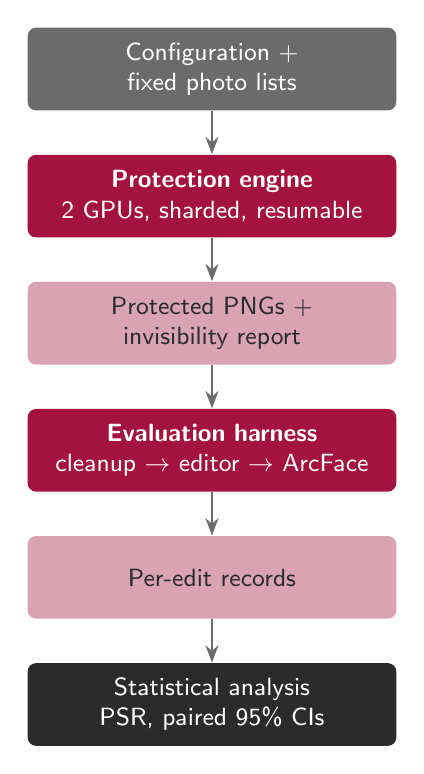
\begin{tikzpicture}[node distance=0.55cm]
            \node[grey,   minimum width=4.6cm, text width=4.4cm] (cfg)  {Configuration + fixed photo lists};
            \node[maroon, minimum width=4.6cm, text width=4.4cm, below=of cfg] (pe) {\textbf{Protection engine}\\2 GPUs, sharded, resumable};
            \node[term,   minimum width=4.6cm, text width=4.4cm, below=of pe] (png) {Protected PNGs + invisibility report};
            \node[maroon, minimum width=4.6cm, text width=4.4cm, below=of png] (eh) {\textbf{Evaluation harness}\\cleanup $\rightarrow$ editor $\rightarrow$ ArcFace};
            \node[term,   minimum width=4.6cm, text width=4.4cm, below=of eh] (rec) {Per-edit records};
            \node[dark,   minimum width=4.6cm, text width=4.4cm, below=of rec] (an) {Statistical analysis\\PSR, paired 95\% CIs};
            \draw[flow] (cfg) -- (pe);
            \draw[flow] (pe) -- (png);
            \draw[flow] (png) -- (eh);
            \draw[flow] (eh) -- (rec);
            \draw[flow] (rec) -- (an);
        \end{tikzpicture}
        \end{adjustbox}
    \end{columns}
\end{frame}

% =========================================================================
% SECTION 3: PRELIMINARY VERIFICATION & DEMONSTRATION
% =========================================================================
\section{Verification \& Demonstration}

\begin{frame}{6. Preliminary Verification \& Quantitative Results}
    \framesubtitle{Experimental Benchmarking \& Comparative Evaluation}
    \begin{table}
        \centering
        \footnotesize
        \renewcommand{\arraystretch}{1.2}
        \begin{tabular}{p{5.6cm} C{2.3cm} C{2.3cm} C{2.6cm}}
            \toprule
            \textbf{Method / Configuration} & \textbf{PSR, no cleanup} & \textbf{PSR, JPEG 75} & \textbf{Photos failing invisibility} \\
            \midrule
            Baseline: unprotected photo & 13.9\% & 10.3\% & -- \\
            Baseline: random noise, same 4/255 budget & 14.9\% & -- & 43 of 100 \\
            Baseline: PhotoGuard at 4/255 (re-implemented) & 81.0\% & 18.3\% & 100 of 100 \\
            Baseline: Mist at 4/255 (re-implemented) & 63.1\% & 21.0\% & 100 of 100 \\
            Ablation: target pull replaced by push-away & 24.3\% & 18.3\% & 0 of 100 \\
            \textbf{Proposed: DiffShield} & \textbf{51.2\%} & \textbf{22.7\%} & \textbf{0 of 100} \\
            \bottomrule
        \end{tabular}
    \end{table}
    \vspace{-0.25cm}
    {\tiny Ablation: same cleanup simulation and denoiser term, but the latent is pushed away from the original instead of toward the target. SD1.5 image-to-image, strength 0.55, 100 test photos, 3 seeds.}

    \begin{block}{Experimental Verification Summary}
        \scriptsize
        \begin{itemize}
            \item \textbf{Quantitative Findings:} DiffShield beats unprotected photos by +37.3 points [+32.7, +42.2] and random noise by +36.3 [+31.9, +40.9] with no visible photo; PhotoGuard and Mist score higher only by visibly altering every photo, and under JPEG 75 DiffShield is ahead of PhotoGuard (+4.3 [+0.7, +8.0]).
            \item \textbf{Verification of Expected Behavior:} without the target pull PSR falls to 24.3\%, confirming it drives the protection; only 1.8\% of edits lose the face, and ArcFace similarity to the person falls from 0.222 to 0.103.
        \end{itemize}
    \end{block}
\end{frame}

\begin{frame}{7. Experimental Visualizations \& Prototype Demonstration}
    \framesubtitle{Result Visualizations, Convergence / Performance Curves \& Live Demo}
    \begin{columns}[T]
        \column{0.48\textwidth}
        \centering
        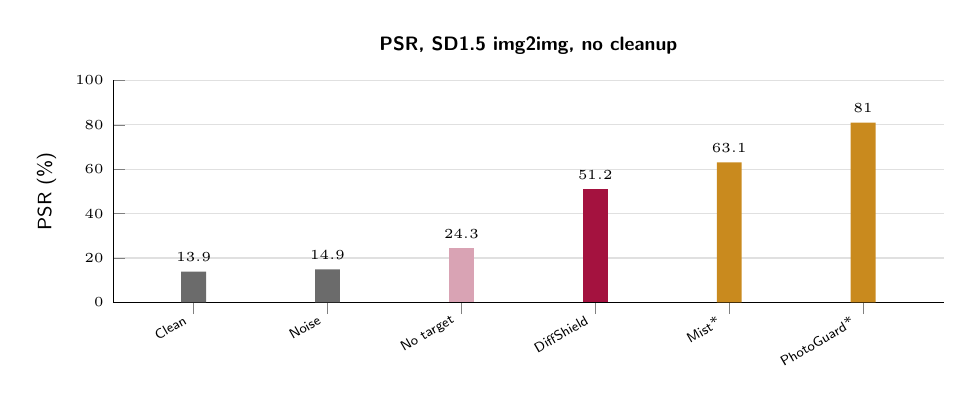
\begin{tikzpicture}
            \begin{axis}[
                width=\linewidth, height=4.4cm, ybar, bar width=9pt, bar shift=0pt,
                ymin=0, ymax=100, xmin=0.4, xmax=6.6,
                xtick={1,...,6}, xticklabels={Clean, Noise, No target, DiffShield, Mist$^{*}$, PhotoGuard$^{*}$},
                x tick label style={font=\tiny, rotate=30, anchor=east},
                y tick label style={font=\tiny}, ylabel={PSR (\%)}, ylabel style={font=\scriptsize},
                title={PSR, SD1.5 img2img, no cleanup}, title style={font=\scriptsize\bfseries},
                nodes near coords, every node near coord/.append style={font=\tiny},
                ymajorgrids, grid style={black!12}, axis lines*=left,
            ]
                \addplot[fill=slateGrey, draw=none] coordinates {(1,13.9) (2,14.9)};
                \addplot[fill=roseMid, draw=none] coordinates {(3,24.3)};
                \addplot[fill=amritaMaroon, draw=none] coordinates {(4,51.2)};
                \addplot[fill=goldAccent, draw=none] coordinates {(5,63.1) (6,81.0)};
            \end{axis}
        \end{tikzpicture}
        {\tiny $^{*}$visibly alter all 100 photos}

        \column{0.48\textwidth}
        \centering
        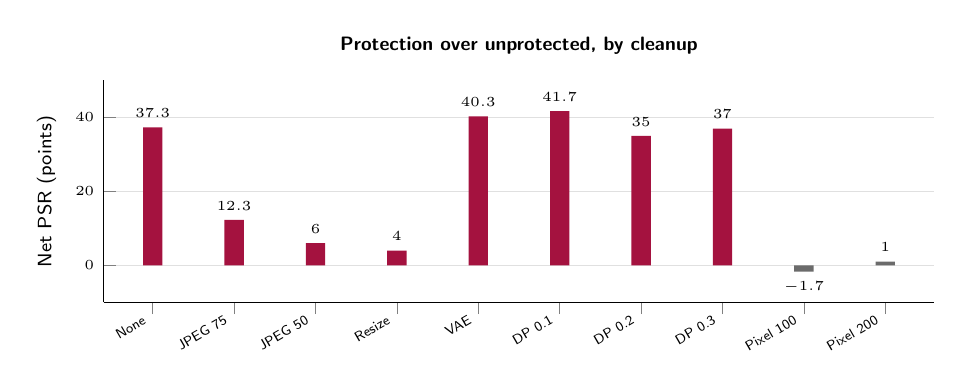
\begin{tikzpicture}
            \begin{axis}[
                width=\linewidth, height=4.4cm, ybar, bar width=7pt, bar shift=0pt,
                ymin=-10, ymax=50, xmin=0.4, xmax=10.6,
                xtick={1,...,10}, xticklabels={None, JPEG 75, JPEG 50, Resize, VAE, DP 0.1, DP 0.2, DP 0.3, Pixel 100, Pixel 200},
                x tick label style={font=\tiny, rotate=30, anchor=east},
                y tick label style={font=\tiny}, ylabel={Net PSR (points)}, ylabel style={font=\scriptsize},
                title={Protection over unprotected, by cleanup}, title style={font=\scriptsize\bfseries},
                nodes near coords, every node near coord/.append style={font=\tiny},
                ymajorgrids, grid style={black!12}, axis lines*=left,
            ]
                \addplot[fill=amritaMaroon, draw=none] coordinates {(1,37.3) (2,12.3) (3,6.0) (4,4.0) (5,40.3) (6,41.7) (7,35.0) (8,37.0)};
                \addplot[fill=slateGrey, draw=none] coordinates {(9,-1.7) (10,1.0)};
            \end{axis}
        \end{tikzpicture}
        {\tiny DP = DiffPure-style (SD1.5); Pixel = pixel-space face DDPM purifier}
    \end{columns}

    \begin{block}{Demonstration Overview}
        \scriptsize Live demo: protect one photo on a GPU (about 4.5 minutes on a T4), edit the original and the protected copy with the same prompt and seed, and show both edits with PSNR/SSIM and each edit's ArcFace similarity to the person (lower = no longer the person).
    \end{block}
\end{frame}

% --- 7 (cont.). BEFORE / AFTER PROTECTION ---
\begin{frame}{7. Experimental Visualizations \& Prototype Demonstration (cont.)}
    \framesubtitle{Edits Before and After Applying DiffShield (same prompt, same seed)}
    \centering
    \imgslot{Unprotected photo}\hfill{\Large\textcolor{amritaMaroon}{$\Rightarrow$}}\hfill
    \imgslot{Edit of unprotected photo}\hspace{0.7cm}
    \imgslot{Protected photo (DiffShield)}\hfill{\Large\textcolor{amritaMaroon}{$\Rightarrow$}}\hfill
    \imgslot{Edit of protected photo}

    \vspace{0.3cm}
    \begin{block}{Reading the Comparison}
        \scriptsize Prompt: ``a person in a suit'' (SD1.5 image-to-image, strength 0.55, same seed for both edits; $\Rightarrow$ = edit with the prompt). The unprotected and protected photos look identical (PSNR $\ge$ 38 dB); DiffShield aims to make the edit of the protected photo stop matching the person, while the edit of the unprotected photo keeps the identity.
    \end{block}
\end{frame}

% =========================================================================
% SECTION 4: TECHNICAL KNOWLEDGE & VIVA VOCE
% =========================================================================
\section{Technical Knowledge}

\begin{frame}{8. Technical Justification, Design Trade-offs \& Insights}
    \framesubtitle{Methodological Rationale, Trade-offs \& Boundary Conditions}
    \begin{columns}[T]
        \column{0.48\textwidth}
        \begin{block}{1. Methodological Justification}
            \scriptsize
            \begin{itemize}
                \item Editors start from the photo's VAE latent; pulling it toward a fixed target gives one consistent direction and derails the edit (without it PSR drops to 24.3\%).
                \item Averaging over random cleanups makes the noise survive them; the one-step DiffPure-style purifier and the denoiser term target diffusion-based cleanup.
            \end{itemize}
        \end{block}

        \begin{block}{2. Design \& Parameter Trade-offs}
            \scriptsize
            \begin{itemize}
                \item Budget (28 tuning photos): 6/255 lifts PSR from 18.9\% to 21.3\% with 1 photo visible; 8/255 gives the same with 12 visible, so 4/255 is kept.
                \item Large denoiser weights gave the worst search trials, so $\eta=0.012$; cost is 274 GPU-seconds per photo.
            \end{itemize}
        \end{block}

        \column{0.48\textwidth}
        \begin{block}{3. Boundary Conditions \& Edge Cases}
            \scriptsize
            \begin{itemize}
                \item Invisibility is enforced on every photo, not on averages; edits with no face count as protected, so the no-face share (1.8\%) is always reported.
                \item Strong under SD-based DiffPure-style cleanup and the VAE round trip; reduced by JPEG and resizing; removed by a pixel-space DDPM purifier.
            \end{itemize}
        \end{block}

        \begin{block}{4. Limitations \& Future Scope}
            \scriptsize
            \begin{itemize}
                \item No protection for SDXL, inpainting or IP-Adapter FaceID; not yet tested against an adaptive attacker; one face recogniser; no human study.
                \item Future: train against pixel-space purifiers and adaptive attackers; identity loss on several face models; SDXL targets.
            \end{itemize}
        \end{block}
    \end{columns}
\end{frame}

% =========================================================================
% REFERENCES & THANK YOU
% =========================================================================
\section{References}
\nocite{*}
\begin{frame}[allowframebreaks]{References}
    \scriptsize
    \bibliographystyle{ieeetr}
    \bibliography{ref}
\end{frame}

\begin{frame}
    \centering
    {\Huge \textbf{\textcolor{amritaMaroon}{Thank You}}} \\[0.4cm]
    {\large \textbf{Questions \& Viva Voce}}
\end{frame}

\end{document}
